\section{Latent Confounding}
\label{sec:latent-confounding}

This section focuses on the more complicated yet realistic case that is 
typically faced by demand modelers, where we have latent confounders that 
affect the treatment assignment of our causal variables of interest, as well as the outcome. 
We first go over a few examples of confounding in transportation analyses, explain 
the challenges that come with such cases, and present a few approaches to 
dealing with this issue, specifically the recent de-confounder technique of 
\citet{wang_2019_blessings}. 
Our application will show how directed acyclic graphs can 
help increase transparency about one's reasoning regarding the number of 
confounders, assumptions for which variables are confounded, and the models 
needed to estimate the causal effects. 
In addition to the application above, we use simplified simulation scenarios to further investigate the usefulness 
and pitfalls of this approach for generating accurate model estimates. 

\subsection{Latent Variable Models}
\label{intro-latent-models}
% TODO: Mechanics of how latent variable models control for unobserved confounding.
Latent variables have been used time and again in different applications of statistical and econometric models in different fields, ranging from epidemiology to transportation.
A latent variable is defined as a covariate not directly observed about subjects in the sample.
Examples of these variables include measurements about happiness, lifestyle, economic expectation, 
morale, among others in many different fields.

Latent variable models are based on the assumption that observed variables are independent conditional on latent variables.
Examples of these models include Integrated Choice and Latent Variable Models, Generalized Linear Latent and Mixed Models,
Factor Analysis Models, and Latent Class Models.

Latent variable models usually rely on collecting indicator/proxy data to infer the levels of latent variable for individuals in a certain sample.
The collection of this data is not always easy or even feasible, mainly due to potential sensitivity of subjects towards some attitudinal questions
This makes it difficult for researchers to collect necessary information that allows for controlling for unobserved factors in models. 

\subsection{Examples of confounding}
\label{sec:confounding-examples}

Confounding occurs when a certain (confounding) variable induces variations in
both the outcome as well as the treatment (policy) variables of interest, 
creating correlation between the treatment and the outcome that is not caused
by the treatment variable itself. When the confounding variable (or variables) is 
observed, we can control for the confounding effect, and there exists many 
methods in the literature for how to do that, including post-stratification,
multiple regression, propensity score methods, etc. It is when the 
confounding variable is unobserved that the problem becomes significantly 
more challenging. 
For an illustration, imagine we're interested in the effect of adding a bike on the mode share of bicycling in a given neighborhood. 
To estimate this effect, one strategy that a modeler may use is to develop a disaggregate mode choice model with a dummy variable for whether a bikelane exists between an individual's trip origin and destination, and then treating the coefficient on this variable as the causal effect of adding a bikelane on the log-odds of choosing to bike. 
The problem with such strategy is that individuals may self-select to live in an area where bicycle infrastructure exists because they have a preference for commuting by bike. 
In other words, if we define an additional variable to encode a person's latent inherent preference for biking, then this variable determines both a person's likelihood for living in an area with an existing bicycle infrastructure, as well as whether that person choose to bike. 
This variable is subsequently expected not to be "balanced" across the treatment and control groups; those who live near a bicycle lane are expected to have higher preference for biking than those who don't. 
Without accounting for this latent confounder, we risk getting very biased estimates 
of the effects of our treatment variable of interest, created by the 
induced variations by the confounder in both the treatment and the outcome 
variable. 



The problem of latent confounding and ommitted variable bias is widely 
acknowledged in the transportation literature, and demand modelers can draw on 
a list of method to account for confouding in some specific circumstances. 
Integrated choice and latent variable (ICLV) models are a way to account for 
the effect of unobserved attitudinal variables which may affect the selection 
of some individuals into some treatment level, as well as an outcome of 
interest. For example, a person's unobserved beliefs and attitudes towards 
being environmentelly friendly may both affect whether she chooses to bike to 
work, as well as whether she lives close to a bike infrastructure, which may 
bias our observational study if we're interested in the effect adding a 
bikelane has on the mode share of bicycles. Those methods, however, rely on 
collecting attitudinal indicators typically obtained by conducting
additional surveys with a sample of the people. This may not be an option in 
many cases; for example, we may not be able to reach the individuals to conduct additional surveys with them. 


\subsection{The deconfounder algorithm}
\label{sec:deconfounder-algo}



One recent method that has been proposed to deal with the problem of latent 
confounding without the need to collect additional data is the deconfounder 
algorithm by \citet{wang_2019_blessings}. The method attempts to control for the 
confouding variable by estimating a "subsitute confounder", a set of variables 
that once controlled for, renders all variation in the treatment variables of 
interest exogenous. The process of applying the method is actually quite 
straightforward and simple. It proceeds as follows:
\begin{itemize}
	\item First, estimate the substitute confounder using any good latent variable 
	model the modeler chooses. The authors suggest estimating a factor model 
	with k factors on the set of covariates the modeler is interested in. 
	\item Second, check the factor model's accuracy using posterior predictive 
	checks (add details). 
	\item Once a sufficiently accurate latent variable model is recovered, use it 
	to estimate an expected value of the latent variable for each observation, 
	and control for this value in the outcome model, alongside the treatment 
	variables and other covariates of interest. 
\end{itemize}



One main assumption of the deconfounder algorithm is that the data at hand 
should have multi-cause confounders, thus the title of the paper, "The 
blessings of multiple causes". In other words, this method works when the 
unobserved confounders affect multiple of the observed causes (or treatment 
variables) of interest, alongside the outcome. This assumption is weaker than 
the one required for ignorability to hold, which requires the absence of both 
single cause and multi-cause confounders for accurate causal inferences. 



\subsection{Case study: Simulation}
\label{sec:deconfounder-simulation}

The purpose of this section is to investigate the effectiveness of the 
deconfounder algorithm \citep{wang_2019_blessings} in adjusting for unobserved 
confounding. We use a simulated mode choice data where travel distance 
linearly confounds both travel time and travel cost. We then mask the travel 
distance data and treat it as an unobserved variable. 


We estimate three models:

\begin{itemize}
	\item Model 1: A multinomial logit with the correct original specification, 
	EXCEPT we ommit the travel distance variable in the specification without 
	trying to adjust for it. This model represents the worst case scenario 
	where a modeler ignores, or is unaware of, unobserved confounding.
	\item Model 2: We use the deconfounder algorithm to try to recover the 
	confounder (travel distance). In this method, we use all the variables in 
	each mode's utility to recover that mode's confounder. This is in line 
	with the approach taken in \citet{wang_2019_blessings}, where they use all the set 
	of observed variables in the factor model to recover a substitute 
	confounder.
	\item Model 3: We use the deconfounder algorithm to try to recover the 
	confounder (travel distance), but this time, we only use travel time and 
	cost in the factor model, instead of all the variables in the utility 
	specification of each mode. By only using what we know are confounded 
	variables to recover the substitute confounder, our goal is to analyze 
	whether we can improve the accuracy of this approach by adopting a more 
	thoughtful approach to hypothesizing on the confounder variables. This can 
	be in the form of building and testing candidate causal graphs that 
	try to illustrate this confounding. 
\end{itemize}


We compare both the estimates of the coefficients on travel time and cost from 
each of those three models to the true estimates used in the simulation, as well as the distribution of the recovered substitute confounder under each of 
models 2 and 3 to the true confounder. The main findings of this exercise are the following:


Using the true variables believed to be confounded (i.e. method 3 where only 
travel time and cost are used to recover the confounder) leads to a better 
recovery of the true confounder. Figure \ref{fig:qq-plot-method-2} and \ref{fig:qq-plot-method-3} show a QQ plot of the true 
and recovered confounders under models 2 and 3 respectively. Looking at those 
figures, one can see that the distribution of the recovered substitute 
confounder under method 3 is closer to that of the true confounder than method 
2. This suggests that it may be better to run the deconfounder algorithm based 
on a hypothesized causal graph, rather than just running it on all the 
observed covariates. Please refer to Section \ref{sec:graph-construction} for how to build plausible causal graphs. 


\begin{figure}
   \centering
   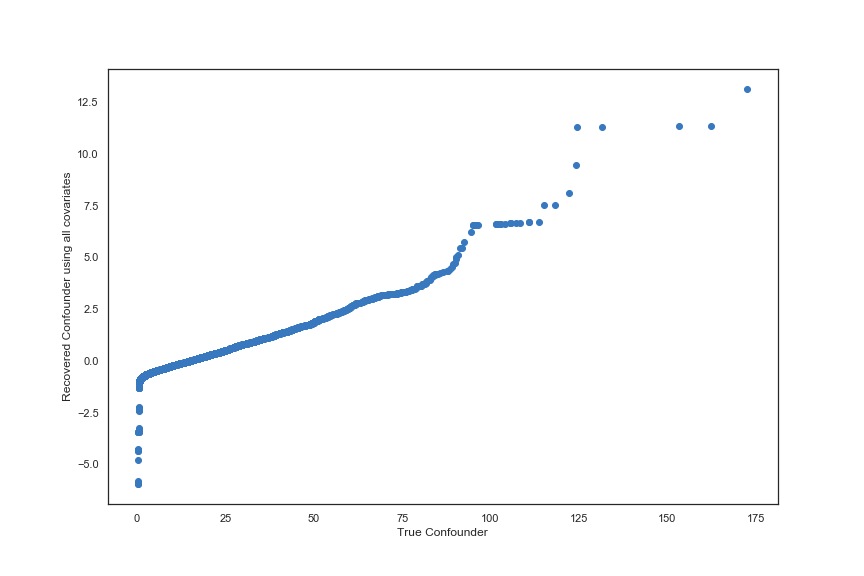
\includegraphics[width=0.5\textwidth]{qq-plot-method-2.png}
   \caption{QQ plot of true confounder against recovered confounder using all covariates}
   \label{fig:qq-plot-method-2}
\end{figure}

\begin{figure}
   \centering
   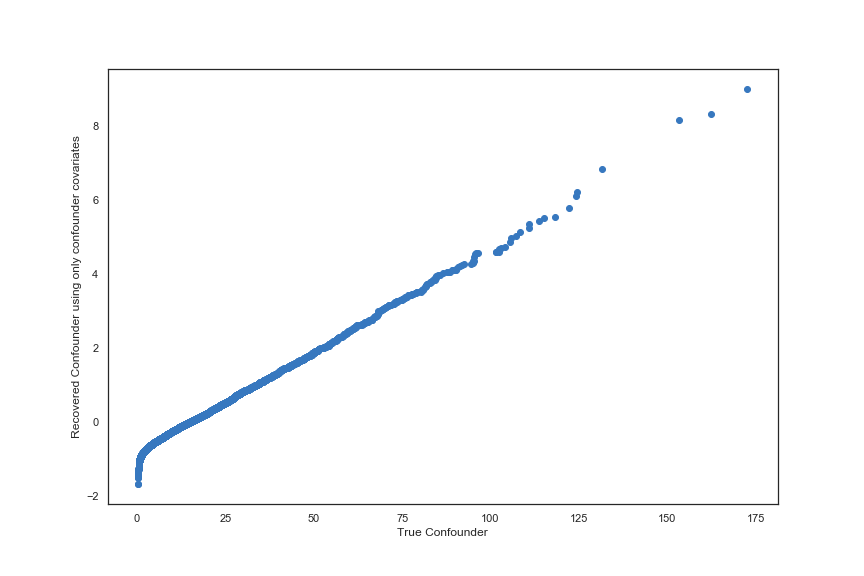
\includegraphics[width=0.5\textwidth]{qq-plot-method-3.png}
   \caption{QQ plot of true confounder against recovered confounder using all covariates}
   \label{fig:qq-plot-method-3}
\end{figure}

% \begin{figure}
% \centering
% \begin{minipage}{.5\textwidth}
%   \centering
%   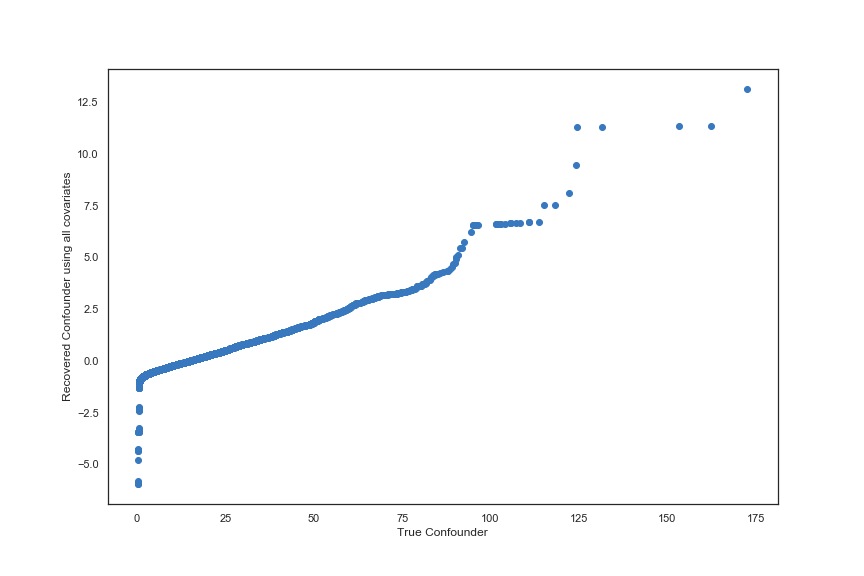
\includegraphics[width=.4\linewidth]{qq-plot-method-2.png}
%   \captionof{figure}{QQ plot of true confounder against recovered confounder using all covariates}
%   \label{fig:qq-plot-method-2}
% \end{minipage}%
% \begin{minipage}{.5\textwidth}
%   \centering
%   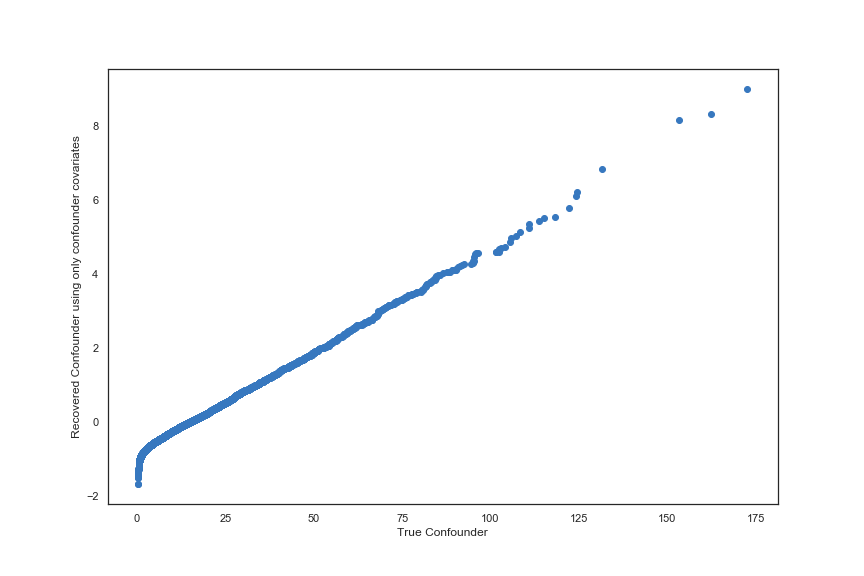
\includegraphics[width=.4\linewidth]{qq-plot-method-3.png}
%   \captionof{figure}{QQ plot of true confounder against recovered confounder using only confounded covariates}
%   \label{fig:qq-plot-method-3}
% \end{minipage}
% \end{figure}


Additionally, and perhaps most importantly, the effectiveness of the 
deconfounder algorithm is very sensitive to small errors and misfits in the 
recovered confounder. Although method 3 returns a relatively good fit of the 
true confounder (based on the QQ plot), the adjusted coefficients on travel 
time and cost do not exhibit any reduction in the bias resulting from 
ommitting the true confounder, and the coefficients on the recovered 
confounder are highly insignificant. This raises questions about the 
usefulness of the deconfounder algorithm in practice. While this limitation 
may raise questions on the usefulness of the deconfounder algorithm, it is 
important to point out that it is not only a by-product of the deconfounder 
algorithm itself. In fact, it is one of the built in characteristic of ommitted
variable bias, and perhaps more broadly, the problem of error-in-variables in 
regression. To illustrate this, suppose we actually observe the true 
confounder variable, but with some white, random guassian noise. Figure \ref{fig:confounder-sensitivity}
shows how the bias in the parameter of interest increases quickly as a 
function of the standard deviation of the random noise. This emphasizes the 
difficulty of recovering unbiased estimates in the presence latent confounders,
and highlights potential limitations with methods that attempt to recover a 
substitute confounder to control for. 

\begin{figure}
   \centering
   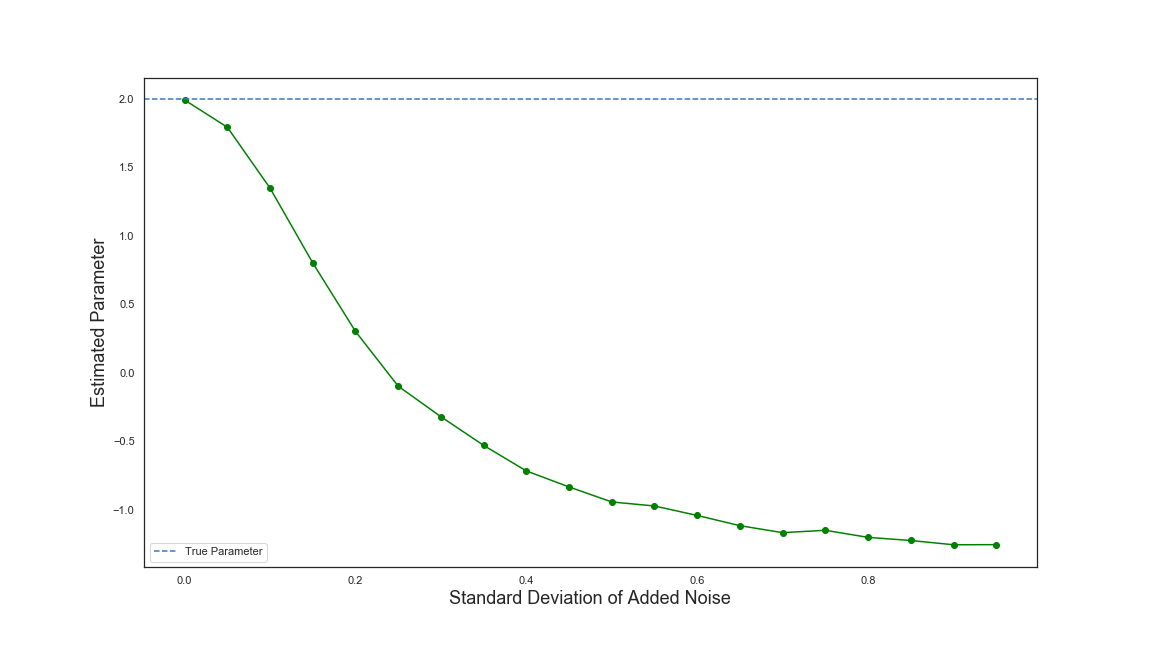
\includegraphics[width=0.5\textwidth]{confounder-sensitivity.png}
   \caption{Sensitivity of causal estimates to random errors in the confounder variable}
   \label{fig:confounder-sensitivity}
\end{figure}

% \begin{figure}
% \centering
% \includegraphics[width=0.5\textwidth]{exa}
% \caption{Sensitivity of causal effect to random noise added to the confounder}
% \label{fig:confounder-sensitivity}
% \end{figure}
